\subsection{Neural Networks}
\label{sec::321_nn}
\cite{weng1992cresceptron} % max pooling
\cite{krizhevsky2012imagenet} % relu
\subsubsection{Fully Connected Neural Network}
The biologically inspired perceptron model \cite{viglione19704} lay the foundation for neural networks and it got extended pretty soon to the multi-layer perceptron model
\cite{ivakhnenko1971polynomial}, which is known today as the fully connected neural network. Due to its similarity to the brain's structure, it is often depicted as in figure \ref{fig::321_fully_connected}, where each orange circle represents a neuron that is connected to its surroundings via simple weights $w_{ij}$, as neurons inside the brain are by axons.
\begin{figure}[h]
	\centering
	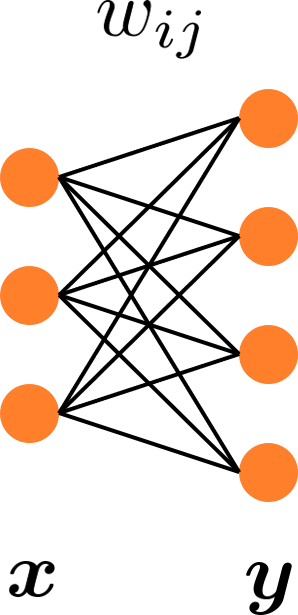
\includegraphics[scale=.28]{chapters/03_background/img/fully_connected.png}
	\caption{Fully connected neural network with three inputs and four outputs. Each orange circle represents what is often referred to as neuron, while the black lines indicate the connections between each neuron.}
	\label{fig::321_fully_connected}
\end{figure}
Mathematically speaking, the feed forward process can be described as a simple matrix multiplication with all weights $\bm{W}$, where the input $\bm{x}$ gets converted to the output $\bm{y}$ via
\begin{align}
	\bm{y} = \bm{W}\bm{x}+\bm{b}
	\label{eq::321_fully_connected}
\end{align}
Therein, the bias $\bm{b}$ can be understood as a shift of isolines that are introduced by hyperplanes. These hyperplanes are learned and expressed by the layer's weights $w_{ij}$ (figure \ref{fig::321_classification}). The output $\bm{y}$, is then further passed through an activation function $f$, and therefore can be compared to the action potential inside a neuron, as it determines the amount by which the next neuron gets excited. This activation function can be anything from a simple step function for classification to a linear function for regression. In practice there are some activation functions that have shown to be of particular use and we will introduce them later in this chapter.
\begin{figure}[h]
	\centering
	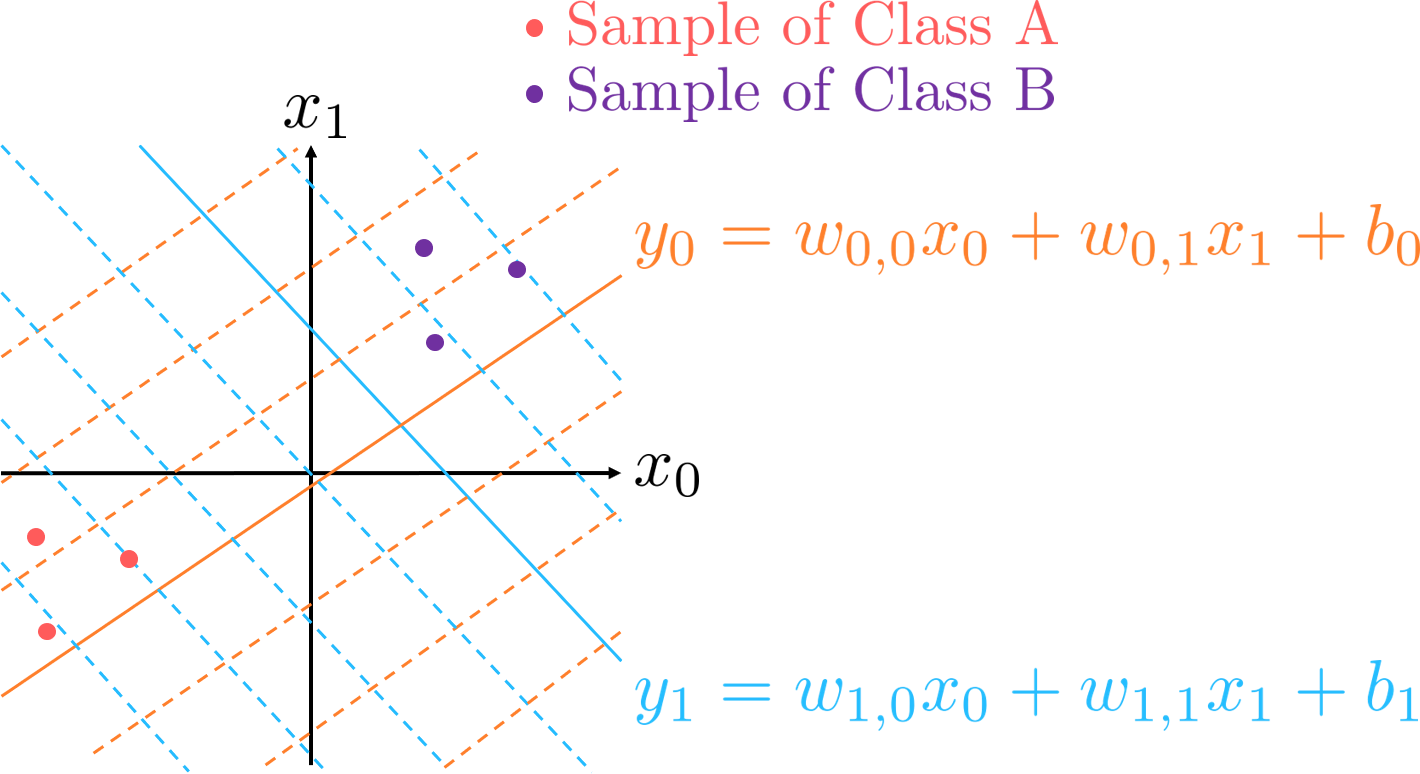
\includegraphics[scale=.28]{chapters/03_background/img/classification.png}
	\caption{Simple interpretation of a fully connected neural network with one layer that takes $\bm{x}=(x_0\,\,x_1)^T$ as input.}
	\label{fig::321_classification}
\end{figure}
\subsubsection{Convolutional Neural Network}
The concept of convolutional neural networks was first inspired by biological structures inside the visual cortex of the human brain. They where first introduced as neocognitron \cite{fukushima1980neocognitron}, and soon after termed convolutional neural networks for their mathematical properties, in that they equal convolutions. Figure \ref{fig::321_convolutional} shows how an input $\bm{x}$ is fed forward through the network architecture across two layers.   
\begin{figure}[h]
	\centering
	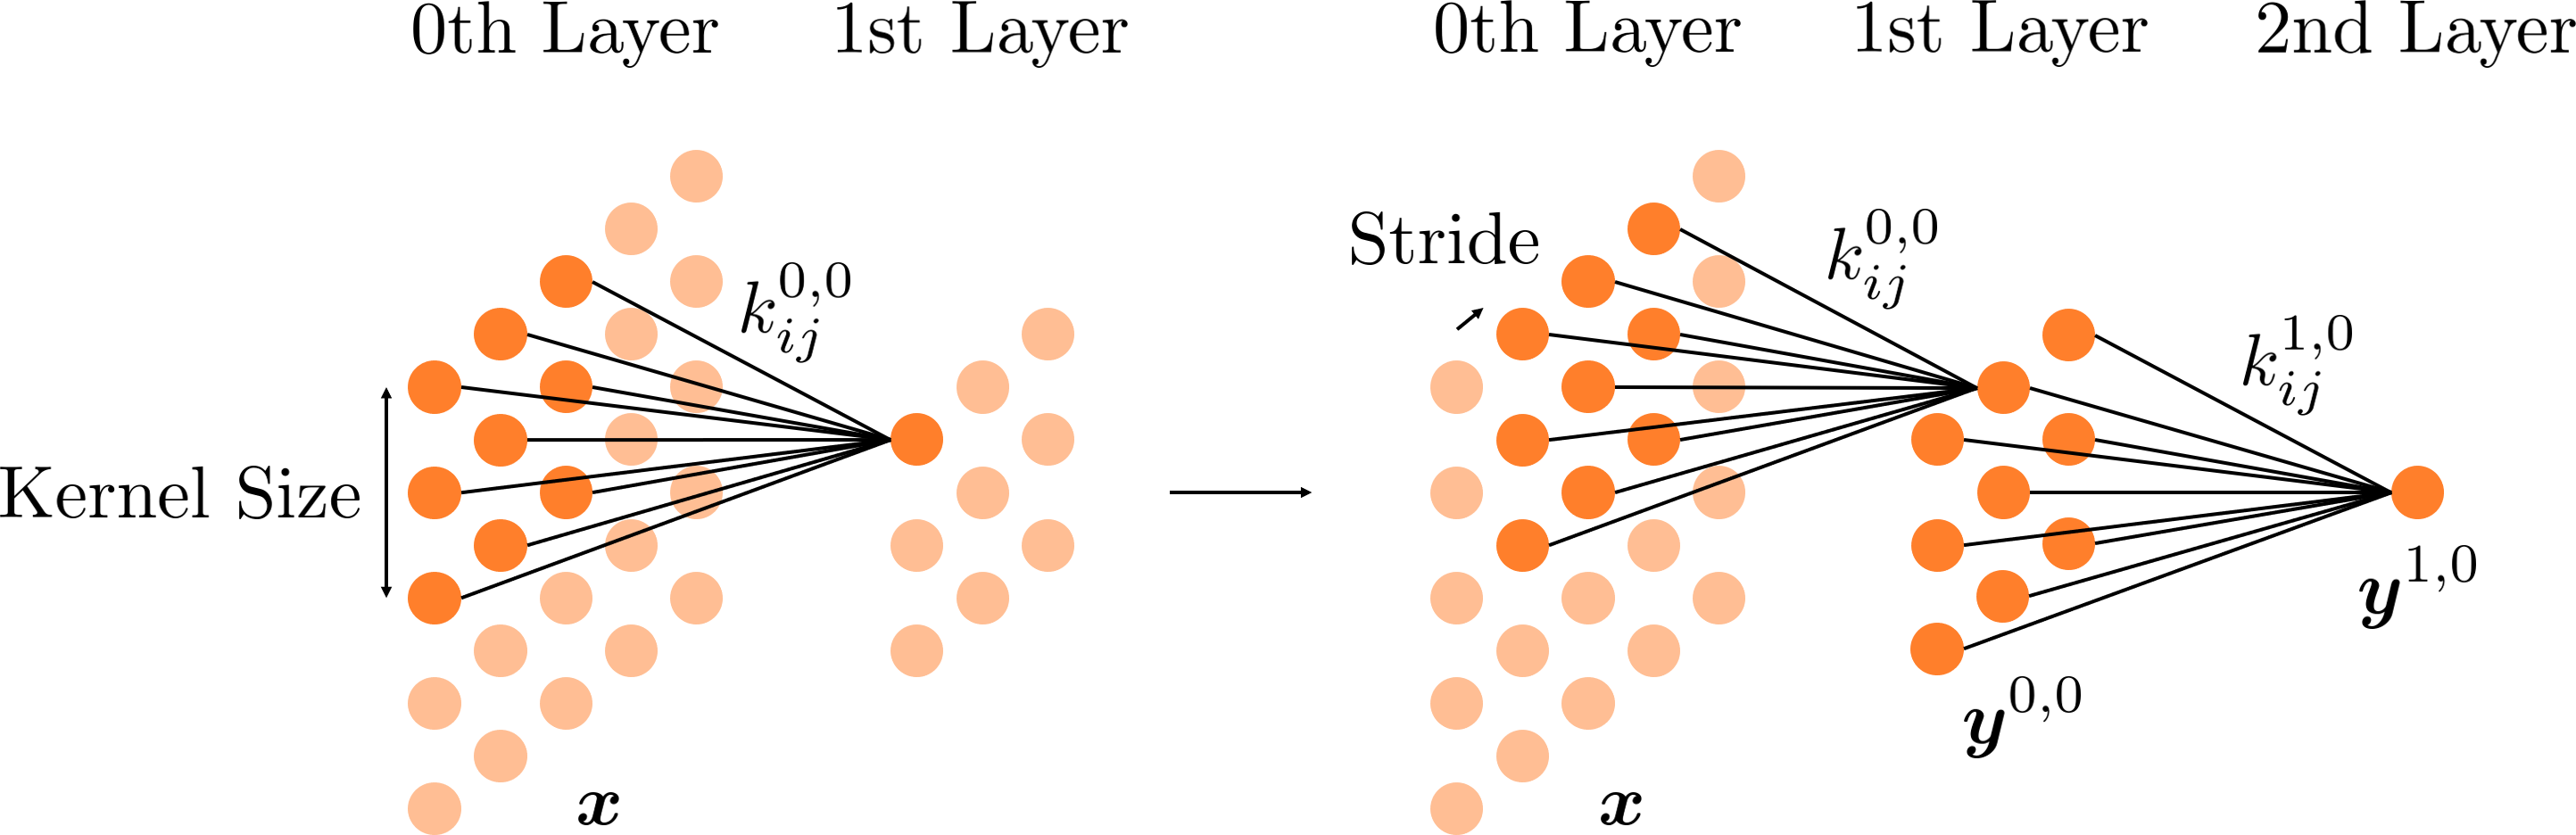
\includegraphics[scale=.28]{chapters/03_background/img/convolutional.png}
	\caption{Convolutional neural network with a total of three layers of which one is the input layer. For visualization, the kernel size is set to be three, and the stride is set to be one.}
	\label{fig::321_convolutional}
\end{figure}
The operation is again visualized by utilizing orange circles, which may be referred to as neurons. These neurons are connected by weights $k^{l,n}_{ij}$, which together constitute the kernel $\bm{k}^{l,n}$ of each convolution. Therein, $l$ stands for the current layer, and $n$ indexes the kernel within a layer, as there may in principle be many different kernels for a single layer. Mathematically speaking, we can formulate the process as follows
\begin{align}
	\bm{y}^{0,0} &= f(\bm{x}*\bm{k}^{0,0}) \\
	\bm{y}^{1,0} &= f(\bm{y}^{0,0}*\bm{k}^{1,0})	
\end{align}
One thing to notice is that the deeper we go, meaning the more layers we have, the more of the initial input contributes to the current activation. This can be seen in figure \ref{fig::321_convolutional}, where each neuron within the first layer only sees a kernel size sized snipped of the original input $\bm{x}$, whereas a neuron within the second layer already sees all of it. 
\cite{zeiler2014visualizing} % understanding neural networks
\subsubsection{Long Short-Term Memory}
\cite{hochreiter1997long} % lstm
\begin{figure}[h]
	\centering
	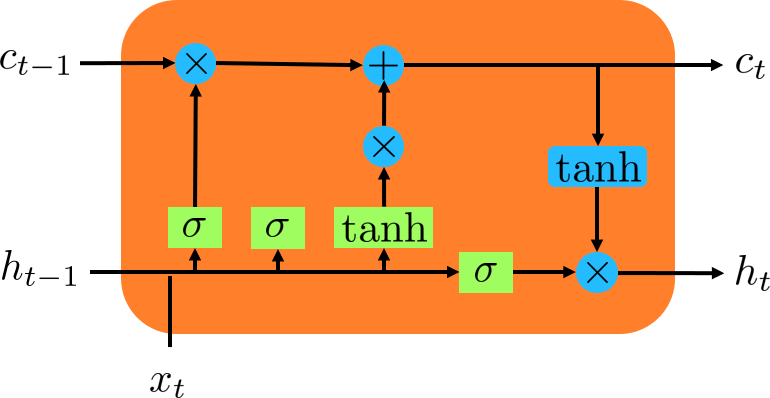
\includegraphics[scale=.28]{chapters/03_background/img/lstm.png}
	\caption{Long short-term memory unit with cell states $\bm{c}_i$, hidden states $\bm{h}_i$, input $\bm{x}_t$, and activation functions $\sigma/\tanh$, as well as addition $+$ and multiplication $\times$ operators.}
	\label{fig::321_lstm}
\end{figure}
\begin{figure}[h]
	\centering
	
\includegraphics[scale=.28]{chapters/03_background/img/lstm_chain.png}
	\caption{Chain of long short-term memory units for temporal understanding of the input sequence $\bm{x}_i$.}
	\label{fig::321_lstm_chain}
\end{figure}
\subsubsection{Backpropagation}
\cite{linnainmaa1970representation}